\chapter{Results and Analysis}\label{chap:Analysis}
The goal of this chapter is to present and analyze the results of the proposed approach. In the first section, results of some baseline methods for the chosen dataset, AFEW-VA are highlighted. Afterwards this work's results are presented and then compared to current state-of-the-art results. Finally, an extensive ablation study is carried out in order to evaluate the impact of design choices.

\section{Baseline Methods}
The authors of the AFEW-VA dataset \citep{Kossaifi:2017:AFEW-VADatabase} provide several baseline experiments for comparison all based on machine-learning methods. Several of these approaches rely on extracted features as input, such as extracting geometrical shapes or appearance features by using Discrete Cosine Transform. Other baseline methods rely on original RGB-Images as input. For fair comparison with our work, we only mention the methods that take as input RGB-images. 
\newline\newline
Table \ref{tab:BaselineMethods} summarizes the results of three baseline methods that take RGB-images as input: Deep Convolutional Neural Network (DCNN), Fine-Tuned DCNN (FT-DCNN) and a ResNet50 model trained from scratch in this work.

\begin{table}[htbp]
\caption[Baseline methods]{The table shows baseline results from \citet{Kossaifi:2017:AFEW-VADatabase} and this work. The FT-DCNN \citep{Kossaifi:2017:AFEW-VADatabase} approach performs best among the basline methods.}
\begin{center}
\begin{tabular}{@{}lcccc@{}}
\toprule
 Method & \begin{tabular}[c]{@{}c@{}}RMSE $\downarrow$\\ Valence\end{tabular} & \begin{tabular}[c]{@{}c@{}}RMSE $\downarrow$\\ Arousal\end{tabular} & \begin{tabular}[c]{@{}c@{}}CORR $\uparrow$\\ Valence\end{tabular} & \begin{tabular}[c]{@{}c@{}}CORR $\uparrow$\\ Arousal\end{tabular} \\ \midrule
DCNN \citep{Kossaifi:2017:AFEW-VADatabase} & 4.1 & 4.6 & 0.17 & 0.25 \\
FT-DCNN \citep{Kossaifi:2017:AFEW-VADatabase} & \textbf{3.7} & \textbf{3.9} & \textbf{0.26} & \textbf{0.31} \\
\begin{tabular}[c]{@{}l@{}}Training from scratch\\ (this work)\end{tabular} & 0.21 & 0.22 & 0.04 & 0.08 \\ \bottomrule
\end{tabular}
\label{tab:BaselineMethods}
\end{center}
\end{table}

\noindent The first method, DCNN, is a model trained from scratch using randomly sampled frames. The second method, FT-DCNN, uses a modified AlexNet \citep{Krizhevsky:2012:AlexNet} architecture that was pre-trained on the ImageNet dataset. This neural network was then further fine-tuned in their work. As shown in Table \ref{tab:BaselineMethods}, FT-DCNN outperforms DCNN. The authors reason that this might be due to not having enough samples for training the model from scratch. Moreover, a ResNet50 architecture, similar to the proposed approach in this work, was trained from scratch to serve as an additional baseline. This approach has a dramatically lower loss in terms of RMSE in comparison to the two previous baselines, but at the same time underperforms in terms of CORR. As the training process aims to lower the RMSE loss, this behavior might be due to a strong overfitting behavior, rendering the model unable to generalize. This would result in a very low CORR.


%%%%%%%%%%%%%%%%%%%%%%%%%%%%%%%%%%%%%%%%%%%%%%%%%%%%%%%%%%%
\section{Results of The Proposed Approach} \label{sec:ResultsProposedApproach}
Since the AFEW-VA dataset has no official validation and test set, as explained in section \ref{sec:TrainValTestSplit}, the data was split subject-independently into a training, validation and test subset. The results presented here are based on the final evaluation of the chosen model on the test set. The chosen model was based on preliminary experiments, conducted on the training and validation set, which helped to find out the optimal hyper-parameters.
\newline\newline
The optimal set hyper-parameters, as explained in section \ref{sec:HyperParameterOptimization}, were used to train the final model in order to predict the outcome in terms of valence and arousal. The averaged training progress is illustrated in Figure \ref{fig:LearningCurveResults} for the two metrics, RMSE and CORR.
\newline 

\begin{figure}[htbp]
  \centering
  \subfloat[Average RMSE during training and validation]{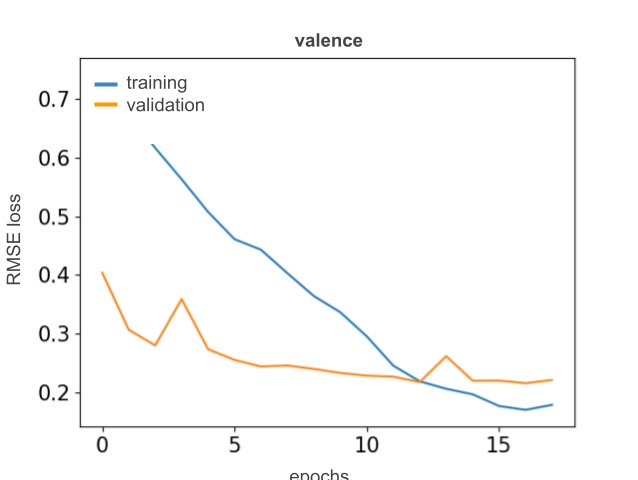
\includegraphics[width=0.7\textwidth]{Figures/Plot_Results_RMSE.png}\label{fig:CurveRMSE}}
  \hfill
  \subfloat[Average CORR during training and validation]{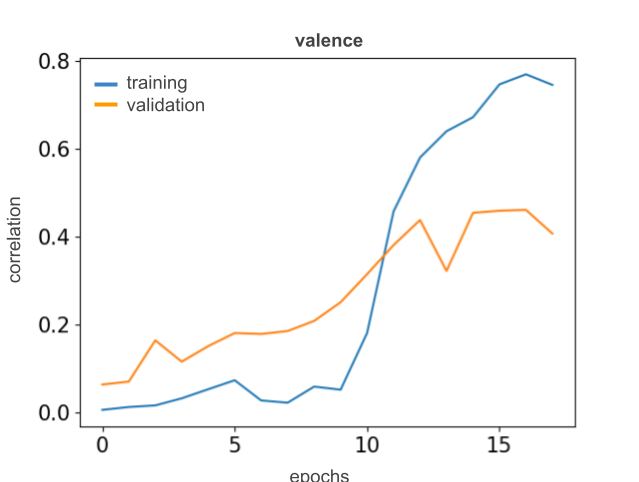
\includegraphics[width=0.7\textwidth]{Figures/Plot_Results_CORR.png}\label{fig:CurveCORR}}
  \caption[Training cures of the proposed approach]{The plots show the learning progress for valence in terms of RMSE and CORR for both, training and validation. Around epoch 11 the validation metrics start to flatten themselves out, while training is still improving. This indicates a tendency of the model overfitting. (Note the slight difference of the y-axis scale in both plots.)}
  \label{fig:LearningCurveResults}
\end{figure}

\noindent A theoretically ideal learning curve would show an exact match between the curves for training and validation. In practice however, the goal is to minimize the difference between training and validation curve over training time and stop training before they diverge from each other. 
\newline\newline
This behaviour can clearly be seen in Figure \ref{fig:LearningCurveResults} as the training and validation curve continuously improve (decrease the RMSE, and increase the CORR) while reducing the distance between them over time. After 3 consecutive epochs, where no improvement was made, the training process gets automatically interrupted and the so far best model is saved. These callbacks are explained in more depth in section \ref{sec:Metrics}.
\newline\newline
All in all, it can be said that the trajectory of the curves gives evidence that the proposed model is a good choice for solving this emotion recognition challenge. The optimal hyper-parameters of the model were then used to conduct a final evaluation on the test subset. The results of this evaluation were averaged over valence and arousal, and are presented in Table \ref{tab:Results}, and its prediction results on the test set are illustrated as a scatter plot in Figure \ref{fig:ScatterPlotValence} and Figure \ref{fig:ScatterPlotArousal}.
\newline

\begin{table}[htbp]
\caption[Results of the proposed approach]{\noha{write \%age difference, not ``excellent" and ``needs improvement".}This table presents the achieved results with the proposed approach. While it provides excellent results for the prediction of valence, it still has room for improvement in terms of arousal.}
\begin{center}
\begin{tabular}{@{}lcccc@{}}
\toprule
\multicolumn{1}{c}{} & \begin{tabular}[c]{@{}c@{}}RMSE $\downarrow$\\ Valence\end{tabular} & \begin{tabular}[c]{@{}c@{}}RMSE $\downarrow$\\ Arousal\end{tabular} & \begin{tabular}[c]{@{}c@{}}CORR $\uparrow$\\ Valence\end{tabular} & \begin{tabular}[c]{@{}c@{}}CORR $\uparrow$\\ Arousal\end{tabular} \\
\midrule
\begin{tabular}[c]{@{}l@{}}VGGFace + RNN\\(this work)\\\end{tabular} & \multicolumn{2}{c}{avg. 0.25} & \multicolumn{2}{c}{avg. 0.50} \\ 
\begin{tabular}[c]{@{}l@{}}VGGFace + RNN\\(this work)\\\end{tabular} & 0.25 & 0.41 & 0.48 & 0.03\\ 
\bottomrule
\end{tabular}
\label{tab:Results}
\end{center}
\end{table}

\begin{figure}[htbp]
  \centering
  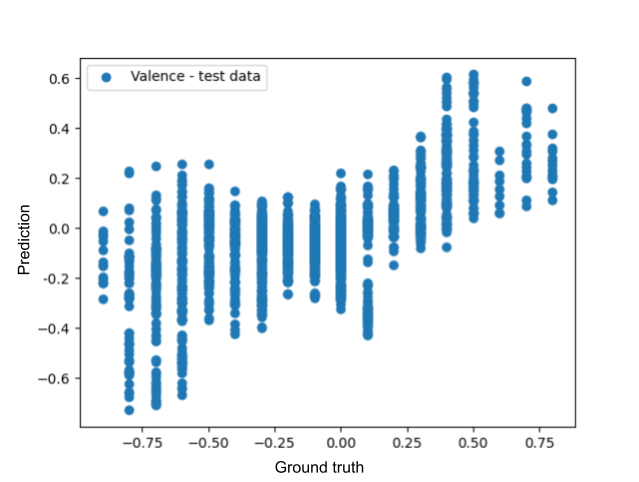
\includegraphics[width=0.7\textwidth]{Figures/ScatterPlot_Valence.png}
  \caption[Scatter plot for valence with the proposed approach]{The scatter plot shows the predicted values for valence mapped against its ground truth. The model is able to predict values very closely to their actual ground truth.}
  \label{fig:ScatterPlotValence}
\end{figure}

\begin{figure}[htbp]
  \centering
  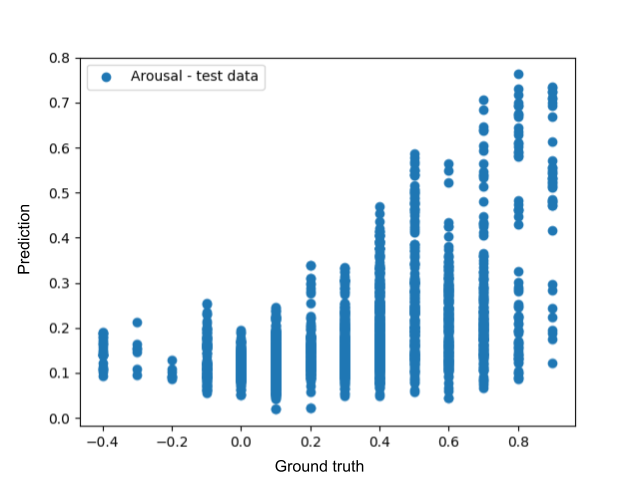
\includegraphics[width=0.7\textwidth]{Figures/ScatterPlot_Arousal.png}
  \caption[Scatter plot for arousal with the proposed approach]{The scatter plot shows the predicted values for arousal mapped against its ground truth. Based on the plot it can be deducted that the model fails to predict accurately for higher ground truth values.}
  \label{fig:ScatterPlotArousal}
\end{figure}

\noindent The results achieved by the 'VGGFace + RNN' approach in this work outperform the baseline methods proposed by \citet{Kossaifi:2017:AFEW-VADatabase} in three out of four metrics. The best baseline method 'FT-DCNN' \citep{Kossaifi:2017:AFEW-VADatabase} approach was outperformed as follows: RMSE valence was decreased by 93\% to 0.25, RMSE arousal was decreased by 89\% to 0.41, and CORR valence was increased by 84\% to 0.48. Only CORR arousal preformed worse which resulted in a decrease of around 90\% to 0.03. However, while the proposed approach outperforms, especially for predicting valence, it still has room for improvement for arousal prediction.  \hl{Explain the results !!}

%%%%%%%%%%%%%%%%%%%%%%%%%%%%%%%%%%%%%%%%%%%%%%%%%%%%%%%%%%%%%
\section{Comparison to State-Of-The-Art} \label{sec:StateOfTheArtComparison}
In this section, three methods achieving state-of-the-art results on the AFEW-VA dataset are presented. The 'CNN + LSTM' \citep{Theagarajan:2018:DeepDriver} method utilized a CNN, pre-trained on the ImageNet dataset, together with a LSTM network which takes into account dynamic variations. Similar to the proposed approach in this thesis, their input data for the model consists of sequences of multiple frames. Furthermore, they used a 3-fold cross-validation approach to evaluate their performance which heavily outperforms the baseline results.
\newline\newline
The other two state-of-the-art methods were proposed by \citet{Handrich:2020:SimultaneousPredVA}. In their 'AFEW-VA DB only' \citep{Handrich:2020:SimultaneousPredVA} method, they only made use of the AFEW-VA database to train and evaluate their Convolution Neural Network (CNN). In their 'Cross-DB validation' \citep{Handrich:2020:SimultaneousPredVA} method, they trained their CNN model on the complete AffectNet \citep{Mollahosseini:2019:AffectNet}, which is a database for facial expression, valence, and arousal computing in the wild. Afterwards they tested their model on the AFEW-VA database. In both methods they used a 5-fold cross-validation where they split data into 70\% training and 30\% testing.
\newline\newline
In Table \ref{tab:StateOfTheArtResults} these state-of-the-art results are compared to the proposed approach, called 'VGGFace + RNN'. It needs to be pointed out that the three authors of the presented results were utilizing different methods for their results evaluation.

\begin{table}[htbp]
\caption[State-of-the-art methods]{In this table, state-of-the-art results are compared to the approach of this work. The emotion recognition approach 'CNN+LSTM' proposed by \citet{Theagarajan:2018:DeepDriver} performs best on all selected criteria.\noha{Enter new results here, not the averaged ones}}
\begin{center}
\begin{tabular}{@{}lcccc@{}}
\toprule
 Method & \begin{tabular}[c]{@{}c@{}}RMSE $\downarrow$\\ Valence\end{tabular} & \begin{tabular}[c]{@{}c@{}}RMSE $\downarrow$\\ Arousal\end{tabular} & \begin{tabular}[c]{@{}c@{}}CORR $\uparrow$\\ Valence\end{tabular} & \begin{tabular}[c]{@{}c@{}}CORR $\uparrow$\\ Arousal\end{tabular} \\ \midrule
CNN + LSTM \citep{Theagarajan:2018:DeepDriver} & \textbf{0.09} & \textbf{0.09} & \textbf{0.64} & \textbf{0.63} \\
AFEW-VA DB only \citep{Handrich:2020:SimultaneousPredVA} & 0.26 & 0.25 & 0.39 & 0.29 \\
Cross-DB validation \citep{Handrich:2020:SimultaneousPredVA} & 0.28 & 0.26 & 0.58 & 0.46 \\
VGGFace + RNN\\(this work) & \multicolumn{2}{c}{avg. 0.25} & \multicolumn{2}{c}{avg. 0.50} \\ \bottomrule
\end{tabular}
\label{tab:StateOfTheArtResults}
\end{center}
\end{table}

\noindent All four methods demonstrate that they are able to outperform the baseline methods. Comparing the outcomes in Table \ref{tab:StateOfTheArtResults} it is visible that the 'CNN + LSTM' method achieves the best results among state-of-the-art methods. 
\newline\newline
However, it needs to be pointed out that the 'CNN + LSTM' approach proposed by \citet{Theagarajan:2018:DeepDriver} and the 'Cross-DB validation' approach proposed by \citet{Handrich:2020:SimultaneousPredVA} were using two different datasets to train their model with. While the proposed 'VGGFace + RNN' and the 'AFEW-VA DB only' approaches were only using a single database. Due to this difference and the fact that the proposed approach is outperforming the 'AFEW-VA DB only' approach, this work's 'VGGFace + RNN' approach can be classified as a state-of-the-art result in emotion recognition in the wild.
\newline\newline
For a future extension of this thesis, it might prove valuable to utilize a second dataset during the training process in order to improve results and beat the results obtained by \citet{Theagarajan:2018:DeepDriver} with their 'CNN + LSTM' approach.


%%%%%%%%%%%%%%%%%%%%%%%%%%%%%%%%%%%%%%%%%%%%%%%%%%%%%%%%%%%%%%%%
\section{Ablation Study}
Ablation Study, in the context of machine learning, involves purposefully removing features or components in order to observe its effects on the system's performance wherein every design choice or module can be included \citep{Lillian:2018:AblationOfARobotsBrain}.
\newline\newline
The experiments presented in the following sections were conducted during the search for optimal hyper-parameters. This means that the results highlighted in this chapter cannot be directly compared to the proposed approach, but give valuable insights that allow to understand the impact of various design decisions during the search for optimal hyper-parameters.

%%%%%%%%%%%%%%%%%%%%%%%%%%%%%%%%%%%%%%%%%%%%%%%%%%%%%%%%%%%%%%%%
\subsection{Network Architecture}
The VGGFace dataset is available pre-trained on one of two different architectures, the ResNet50 and VGG16 architecture. Both models have achieved outstanding performance in machine learning competitions. The difference being that ResNet50 is a more deep-layered neural network, while VGG16 contains more parameters to be trained. A comparison of both can be seen in Table \ref{tab:ResNet50vsVGG16}.

\begin{table}[htbp]
\caption[Ablation study: ResNet50 vs. VGG16]{The table shows results of the fine-tuning of the VGG16 and ResNet50 architecture. Both architectures performed similar, and can thus be considered equally suitable for emotion recognition}
\begin{center}
\begin{tabular}{@{}lcccc@{}}
\toprule
\multicolumn{1}{l}{Method} & \begin{tabular}[c]{@{}c@{}}RMSE $\downarrow$\\ Valence\end{tabular} & \begin{tabular}[c]{@{}c@{}}RMSE $\downarrow$\\ Arousal\end{tabular} & \begin{tabular}[c]{@{}c@{}}CORR $\uparrow$\\ Valence\end{tabular} & \begin{tabular}[c]{@{}c@{}}CORR $\uparrow$\\ Arousal\end{tabular} \\ \midrule
with ResNet50 & 0.21 & 0.20 & 0.15 & 0.21 \\
with VGG16 & 0.20 & 0.19 & 0.15 & 0.22 \\ \bottomrule
\end{tabular}
\label{tab:ResNet50vsVGG16}
\end{center}
\end{table}

\noindent The comparison above shows that the VGG16 model architecture is slightly outperforming ResNet50. However, due to multi-phase fine-tuning approach utilized during this experiment, there are differences in the amount of parameters added during the process of unfreezing additional layers in each phase. Due to this inherent difference a slight change in the outcomes should not allow to draw conclusions about having a better architecture. As a result, this work regards both architecture as an equally valid choice. 
\newline\newline
The final decision fell on the ResNet50 architecture to be utilized for further studies, for two reasons: 1) ResNet50's novel skip connection approach actively mitigates the vanishing gradient problem, and 2) Due to memory constraints, the number of parameters of ResNet50 is with around 25.5 million more advantageous than VGG16 with its 138 million parameters.


%%%%%%%%%%%%%%%%%%%%%%%%%%%%%%%%%%%%%%%%%%%%%%%%%%%%%%%%%%%%%%%%
\subsection{Multi- Phase Fine-Tuning}
Multi-Phase Fine-Tuning is an approach aiming to increase the performance of a pre-trained neural network for a specific challenge at hand. While a conventional fine-tuning approach consists of unfreezing all the needed layers at once at the beginning of the training, the Multi-Phase Fine-Tuning involves the successive unfreezing of groups of layers. The neural network's to be updated weights were increased over several phases. \citet{Sarhan:2020:MultiPhaseFineTuning} show that Multi-Phase Fine-Tuning results in higher classification accuracy, while requiring less training time in comparison to earlier fine-tuning approaches.
\newline\newline
The results achieved in this Master thesis were achieved with the Multi-Phase Fine-Tuning (FT) approach and can be seen in Section \ref{sec:ResultsProposedApproach}. In the following experiment, conducted during the search for optimal hyper-parameters, the two strategies Single-Phased FT and Multi-Phased FT are contrasted. \newline

\begin{figure}[htbp]
  \centering
  \subfloat[Single-Phase FT]{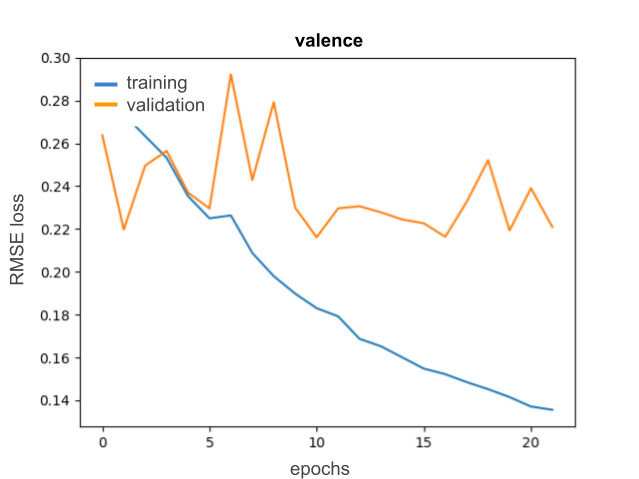
\includegraphics[width=0.7\textwidth]{Figures/Plot_AblationStudy_SinglePhaseFT.png}\label{fig:SinglePhaseFTall}}
  \hfill
  \subfloat[Multi-Phase FT]{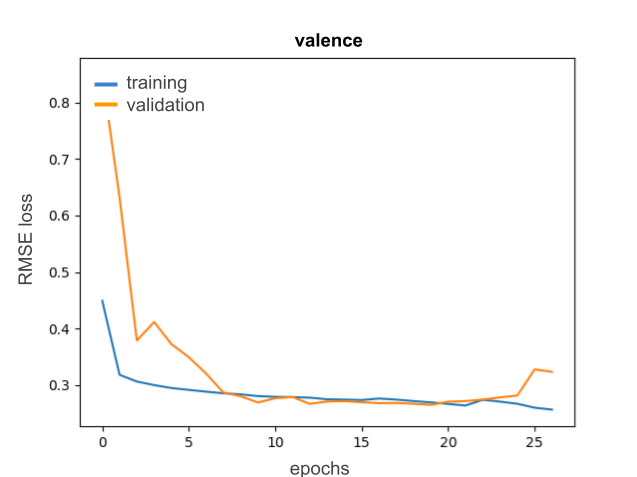
\includegraphics[width=0.7\textwidth]{Figures/Plot_AblationStudy_MultiPhaseFT.png}\label{fig:MultiPhaseStep2}}
  \caption[Ablation study: Multi-Phase FT loss curves]{The graphs show a comparison of the training and validation RMSE loss curves for Single-Phase FT and Multi-Phase FT. Multi-Phase FT reveals a better and smoother convergence between training and validation curve. (Note the difference of the x-axis and y-axis scale in both plots.)}
  \label{fig:SPFTvsMPFT}
\end{figure}

\noindent In Figure \ref{fig:SPFTvsMPFT}, it can clearly be seen in the RMSE loss curve for Single-Phase FT that the 'test' curve representing the validation loss is not following the 'train' curve in its downward trend. This is a strong indication for a overfitting behavior as the model is not able to generalize from the training data. Unlike the RMSE loss curve for Multi-Phase FT where the training and validation losses are continuously decreasing and converging with each other. This observation is also reflected in the achieved validation results presented in Table \ref{tab:SPFTvsMPFT}, where the Multi-Phase FT clearly outperforms the Single-Phase FT approach in terms of RMSE and CORR.

\begin{table}[H]
\caption[Ablation study: Multi-Phase FT results]{The table contains a comparison of the fine-tuning strategies Single-Phase FT with Multi-Phase FT. Validation results confirm that Multi-Phase FT outperforms Single-Phase FT.}
\begin{center}
\begin{tabular}{@{}lcccc@{}}
\toprule
\multicolumn{1}{l}{Methods} & \begin{tabular}[c]{@{}c@{}}RMSE $\downarrow$\\ Valence\end{tabular} & \begin{tabular}[c]{@{}c@{}}RMSE $\downarrow$\\ Arousal\end{tabular} & \begin{tabular}[c]{@{}c@{}}CORR $\uparrow$\\ Valence\end{tabular} & \begin{tabular}[c]{@{}c@{}}CORR $\uparrow$\\ Arousal\end{tabular} \\ \midrule
\begin{tabular}[c]{@{}l@{}}Single-Phase FT \end{tabular} & 0.24 & 0.24 & 0.13 & 0.15 \\
\begin{tabular}[c]{@{}l@{}}Multi-Phase FT \end{tabular} & 0.24 & \textbf{0.22} & \textbf{0.38} & \textbf{0.46} \\ \bottomrule
\end{tabular}
\label{tab:SPFTvsMPFT}
\end{center}
\end{table}


%%%%%%%%%%%%%%%%%%%%%%%%%%%%%%%%%%%%%%%%%%%%%%%%%%%%%%%%%%%%%%%%
\subsection{MTCNN (Multi-task Cascaded Convolutional Neural Network)}
As already outlined in Section \ref{sec:FaceDetection}, the pre-trained MTCNN module was utilized to detect faces in an image and to determine the face's bounding box. 
\newline\newline
Next to the actual performance increase due to the detection of a person's face, it is important to highlight the failure rate of such a module. Based on the AFEW-VA dataset, consisting of 30.051 frames, the MTCNN module failed to detect a person's face in 961 cases. This equals a failure rate of 3.2 percent. 
\newline\newline
To put this into perspective, results were compared to the failure rate of the FaceReader \citep{Noldus:2020:Facereader} application, a production-ready software tool that assists researcher in the automatic recognition of facial expressions. Based on a sample taken from the AFEW-VA database, FaceReader had a failure rate of 33 percent. This is likely due to the fact that their product is designed for laboratory conditions (e.g. they recommend the camera be placed slightly below eye-level and the face be fully illuminated, without any shadow). In summary, it can be said that the MTCNN's face detection rate of 96.8 percent on in-the-wild data is excellent.
\newline\newline
The pipeline for the usage of the MTCNN module includes the following steps: First, faces inside an image were detected. Second, the primary face was selected. Third, the face was cropped along its bounding box and fed into the neural network. For frames where the detection of a face was not possible, the image was discarded as it wouldn't have been possible to determine landmark positions without a bounding box. 
\newline\newline
The following table compares training results achieved with the MTCNN model during the search for optimal hyper-parameters.

\begin{table}[htbp]
\caption[Ablation study: MTCNN results]{The table compares results from training a neural network with and without the MTCNN module. The model is responsible for detecting a person's face and allowing the face to be extracted. As seen in the table the neural network clearly performs better with MTCNN}
\begin{center}
\begin{tabular}{@{}lcccc@{}}
\toprule
\multicolumn{1}{l}{Methods} & \begin{tabular}[c]{@{}c@{}}RMSE $\downarrow$\\ Valence\end{tabular} & \begin{tabular}[c]{@{}c@{}}RMSE $\downarrow$\\ Arousal\end{tabular} & \begin{tabular}[c]{@{}c@{}}CORR $\uparrow$\\ Valence\end{tabular} & \begin{tabular}[c]{@{}c@{}}CORR $\uparrow$\\ Arousal\end{tabular} \\ \midrule
with MTCNN & 0.24 & \textbf{0.24} & \textbf{0.13} & \textbf{0.15} \\
without MTCNN & 0.24 & 0.26 & -0.02 & 0.08 \\ \bottomrule
\end{tabular}
\label{tab:ExperimentMTCNN}
\end{center}
\end{table}

\noindent In summary, the MTCNN module used for face detection and bounding boxing clearly contributed to the overall improvement of the model's performance. Furthermore, the detection of the bounding box provides a necessary input for the detection of landmark points.

%%%%%%%%%%%%%%%%%%%%%%%%%%%%%%%%%%%%%%%%%%%%%%%%%%%%%%%%%%%%%%%%
\subsection{Facial Landmarks}
Detecting a person's facial landmarks and utilizing them to improve emotion recognition is a current research trend, as was shown in state-of-the-art literature, for example by \citet{Gupta:2018:FacialLandmarks-1} and \citet{Tautkute:2018:FacialLandmarks-2} in 2018. One of the most widely used and accurate approaches for the detection is called an Active Appearance Model \citep{Cootes:2001:ActiveAppearanceModel}. Even though it is described by \citet{Gao:2010:ActiveAppearanceModels} as a very suitable approach for the extraction of compact features, it doesn't satisfy real-time requirements due to its time consuming fitting process.
\newline\newline
Such an approach could not have satisfied the real-time requirements for in the wild use cases set by PPI AG. Instead an algorithm based on an ensamble of regression trees, introduced by \citet{Kazemi:2014:ShapePredictor}, able to predict 68 facial landmarks in milliseconds was utilized.
\newline\newline
Landmarks obtained from the algorithm were fed into the neural network in one of the following four ways, also illustrated in Figure \ref{fig:LandmarksImages}: 

\begin{enumerate}
    \item \textbf{Direct Overlay} \newline \indent Each landmark point was drawn as an overlay onto the face's image with full opacity.
    \item \textbf{Soft Overlay} \newline \indent Each landmark point was drawn as an overlay onto the face's image with an opacity of 0.2.
    \item \textbf{Heatmap Overlay} \newline \indent Landmark points were converted into a heatmap and applied as an overlay onto the face's image.
    \item \textbf{Separate 2D Mask} \newline \indent Each landmark point is represented on a gray-scale image by a pixel value between 0 and +1. A gaussian filter was applied to blur the image.
\end{enumerate}

\noindent Through the application of an overlay on top of the actual image, actual pixels of the face's input image were modified. This wasn't necessary with the 'Separate 2D Mask' approach, as the landmarks are captured in a separate gray-scale image that was fed into a second input stream of the neural network.

\begin{figure}[htbp]
  \begin{center}
  \subfloat[Landmarks as dots]{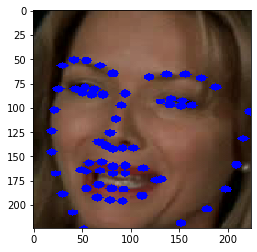
\includegraphics[width=0.4\textwidth]{Figures/landmarks_as_dots.png}}
  \hfill
  \subfloat[Landmarks as soft overlay]{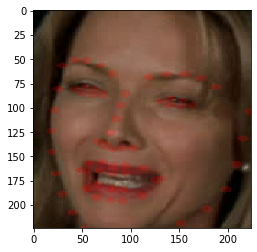
\includegraphics[width=0.4\textwidth]{Figures/landmarks_as_softOverlay.png}}
  \hfill
  \subfloat[Landmarks as heatmap overlay]{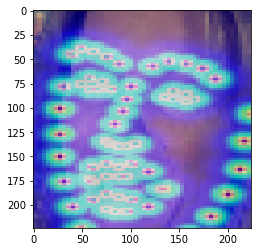
\includegraphics[width=0.4\textwidth]{Figures/landmarks_as_heatmap.png}}
  \hfill
  \subfloat[Separate 2D Mask]{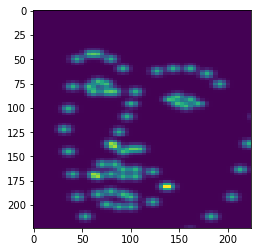
\includegraphics[width=0.4\textwidth]{Figures/landmarks_as_heatmap_in_mask.png}}
  \caption[Ablation study: Landmark visualizations]{The figure shows various ways of how landmarks were applied to the face image.}
  \label{fig:LandmarksImages}
  \end{center}
\end{figure}

\noindent An intuitive way of applying facial landmarks to an image is to use the dots as an overlay. However, it became clear that such doing would make important information in the underlying image invisible to the neural network. Instead different approaches were tried to remedy this implication, like a soft overlay or a heatmap overlay. Eventually, it turned out that keeping the face's image completely pristine while using a separate 2D mask for facial landmarks delivered the best results. These results are compared visually in Figure \ref{fig:LandmarksVisualComparison} and through the RMSE and CORR metrics in Table \ref{tab:LandmarksComparison}.\newline

\begin{figure}[htbp]
  \begin{center}
  \subfloat[Landmarks as dots]{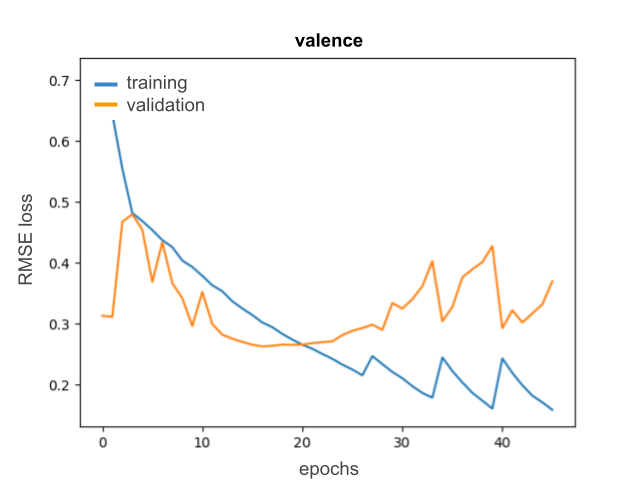
\includegraphics[width=0.5\textwidth]{Figures/Plot_AblationStudy_LandmarksDots.png}}
  \hfill
  \subfloat[Landmarks as heatmap overlay]{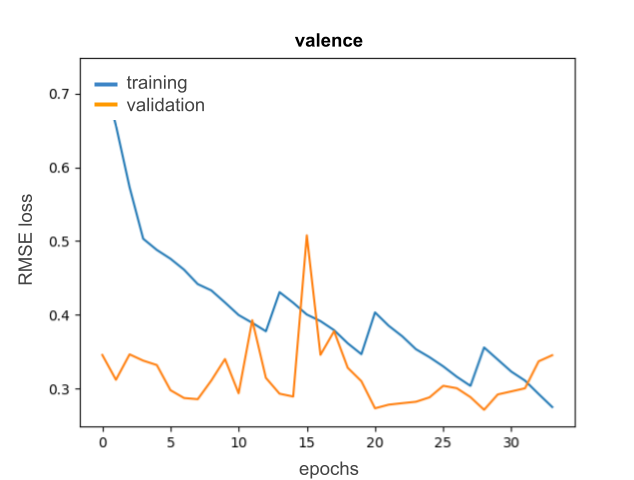
\includegraphics[width=0.5\textwidth]{Figures/Plot_AblationStudy_LandmarksHeatmap.png}}
  \hfill
  \subfloat[Landmarks as soft overlay]{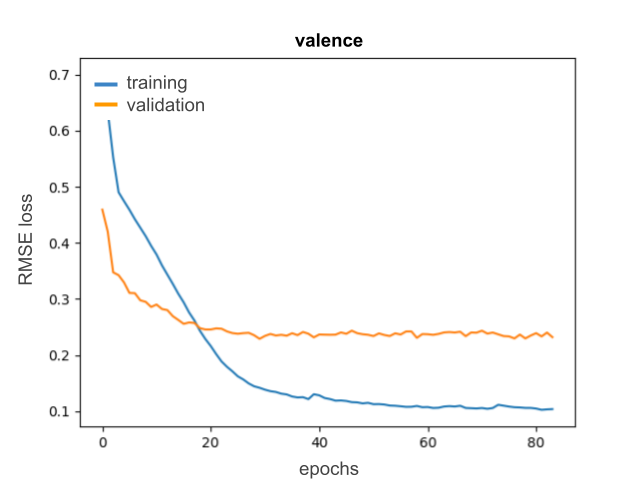
\includegraphics[width=0.5\textwidth]{Figures/Plot_AblationStudy_LandmarksSoftAttention.png}}
  \hfill
  \subfloat[Landmarks as separate mask]{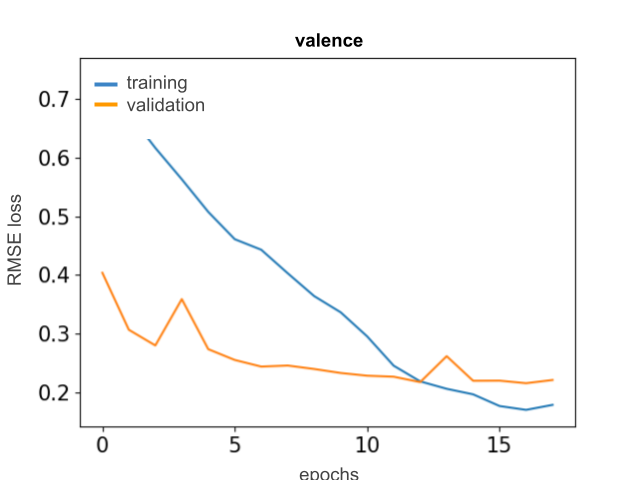
\includegraphics[width=0.5\textwidth]{Figures/Plot_AblationStudy_LandmarksMask.png}}
  \caption[Ablation study: Landmark methods loss curves]{The plots show for each landmark method a training and validation loss curve in terms of RMSE. A trend becomes visible: The more of a face is covered by landmarks, the worse the convergence between training and validation curve. (Note the difference of the x-axis and the y-axis scale in all plots.)}
  \label{fig:LandmarksVisualComparison}
  \end{center}
\end{figure}

\begin{table}[htbp]
\caption[Ablation study: Landmark methods results]{The table displays a result comparison between the tested landmark methods. The best performance could be achieved by feeding a separate 2D mask into the neural network.}
\begin{center}
\begin{tabular}{lcccc}
\hline
\multicolumn{1}{l}{Methods} & \begin{tabular}[c]{@{}c@{}}RMSE $\downarrow$\\ Valence\end{tabular} & \begin{tabular}[c]{@{}c@{}}RMSE $\downarrow$\\ Arousal\end{tabular} & \begin{tabular}[c]{@{}c@{}}CORR $\uparrow$\\ Valence\end{tabular} & \begin{tabular}[c]{@{}c@{}}CORR $\uparrow$\\ Arousal\end{tabular} \\ \hline
\begin{tabular}[c]{@{}l@{}}Landmarks as dots\end{tabular} & 0.21 & 0.22 & 0.02 & 0.00 \\
\begin{tabular}[c]{@{}l@{}}Landmarks as heatmap \end{tabular} & 0.22 & 0.22 & 0.00 & 0.00 \\
\begin{tabular}[c]{@{}l@{}}Landmarks as soft overlay\end{tabular} & \textbf{0.19} & \textbf{0.20} & 0.08 & 0.07 \\
\begin{tabular}[c]{@{}l@{}}Landmarks as separate 2D Mask\end{tabular} & 0.24 & 0.24 & \textbf{0.10} & \textbf{0.20} \\ \bottomrule
\end{tabular}
\label{tab:LandmarksComparison}
\end{center}
\end{table}

\noindent All in all, it can be summarized that leaving the face's image untouched, while feeding facial landmarks separately into the neural network has the highest potential of increasing the model performance.


%%%%%%%%%%%%%%%%%%%%%%%%%%%%%%%%%%%%%%%%%%%%%%%%%%%%%%%%%%%%%%%%
\subsection{Regularization}
Regularization techniques are generally used to introduce error and/or randomness during the training process which makes training for the model harder, in the hope of a better generalization which in turn results in a better performance during validation/testing of the model. The experiments presented in this section were conducted during the search for optimal hyper-parameters.

\subsubsection{Dropout}
The following Figure \ref{fig:AblationNoDropout} highlights the effects of a removal of the dropout in the custom added classifier on the RMSE metric.\newline

\begin{figure}[htbp]
  \centering
  \subfloat[With Dropout]{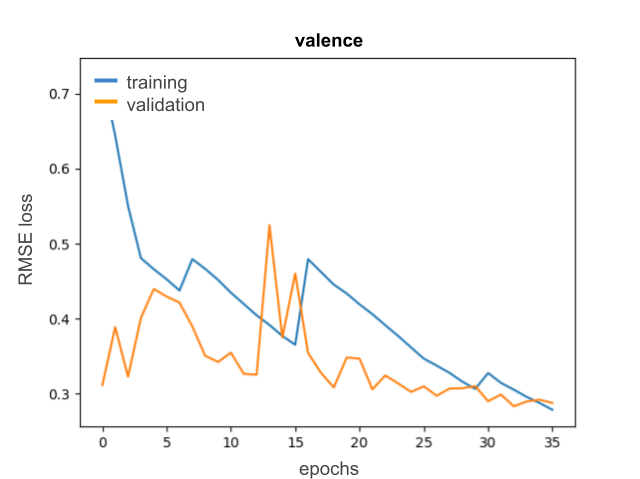
\includegraphics[width=0.7\textwidth]{Figures/Plot_AblationStudy_NoDataAug.png}\label{fig:WithDropout}}
  \hfill
  \subfloat[No Dropout]{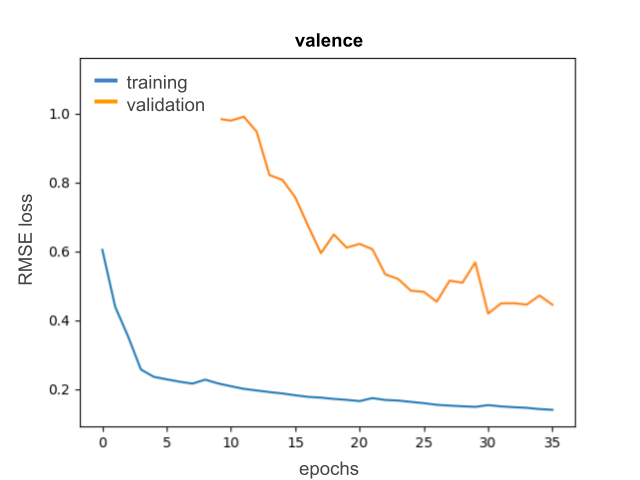
\includegraphics[width=0.7\textwidth]{Figures/Plot_AblationStudy_NoDropout.png}\label{fig:NoDropout}}
  \caption[Ablation Study: Dropout loss curve]{The graphs show the loss curves in terms of training and validation RMSE for a) with dropout and b) no dropout. The removal of Dropout from the classifier resulted in a spike in terms of validation loss. (Note the difference of the y-axis scale in both plots.)}
  \label{fig:AblationNoDropout}
\end{figure}

\noindent As expected, due to the missing regularization effect of the Dropout layers, the validation loss curve unveiled a significantly higher validation loss. This is also confirmed by the results presented in Table \ref{tab:MPFTDropout}, where the removal of Dropout layers perform significantly worse in all four measured metrics.


\begin{table}[htbp]
\caption[Ablation study: Dropout results]{The table shows a result comparison between the application of dropout and its removal. It further highlights that the application of dropout leads to a performance increase in all four categories.}
\begin{center}
\begin{tabular}{@{}lcccc@{}}
\toprule
\multicolumn{1}{l}{Methods} & \begin{tabular}[c]{@{}c@{}}RMSE $\downarrow$\\ Valence\end{tabular} & \begin{tabular}[c]{@{}c@{}}RMSE $\downarrow$\\ Arousal\end{tabular} & \begin{tabular}[c]{@{}c@{}}CORR $\uparrow$\\ Valence\end{tabular} & \begin{tabular}[c]{@{}c@{}}CORR $\uparrow$\\ Arousal\end{tabular} \\ \midrule
\begin{tabular}[c]{@{}l@{}}Multi-Phased FT\\(with Dropout)\end{tabular} & \textbf{0.29} & \textbf{0.25} & \textbf{-0.10} & \textbf{0.12} \\
\begin{tabular}[c]{@{}l@{}}Multi-Phased FT\\ without Dropout\end{tabular} & 0.47 & 0.49 & -0.11 & 0.03 \\ \bottomrule
\end{tabular}
\label{tab:MPFTDropout}
\end{center}
\end{table}

\subsubsection{Batch Normalization}
Figure \ref{fig:AblationNoBatchNorm} illustrates the effects of a removal of the classifier's BatchNormalization layer on the RMSE metric for valence.\newline

\begin{figure}[htbp]
  \begin{center}
  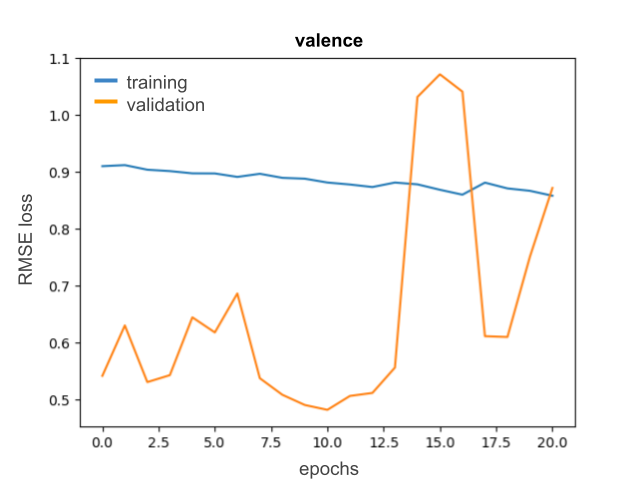
\includegraphics[angle=0, width=0.7\textwidth]{Figures/Plot_AblationStudy_BatchNorm.png}
  \caption[Ablation study: BatchNormalization loss curve]{The graph depicts the training and validation loss curves in terms of RMSE for the removal of Batch Normalization. Due to this the validation loss curve behaviour turned out to be very erratic.}
  \label{fig:AblationNoBatchNorm}
  \end{center}
\end{figure}         

\noindent Due to the erratic behavior of the validation loss in terms of RMSE and the general upward trend of the validation loss already indicate a bad performance. The expected performance degradation is presented in Table \ref{tab:MPFTNoBatchNorm}

\begin{table}[htbp]
\caption[Ablation study: BatchNormalization results]{The table compares the results achieved with the application of BatchNormalization with its removal. It emphasises that BatchNormalization can increase the overall performance of the neural network.}
\begin{center}
\begin{tabular}{@{}lcccc@{}}
\toprule
\multicolumn{1}{l}{Methods} & \begin{tabular}[c]{@{}c@{}}RMSE $\downarrow$\\ Valence\end{tabular} & \begin{tabular}[c]{@{}c@{}}RMSE $\downarrow$\\ Arousal\end{tabular} & \begin{tabular}[c]{@{}c@{}}CORR $\uparrow$\\ Valence\end{tabular} & \begin{tabular}[c]{@{}c@{}}CORR $\uparrow$\\ Arousal\end{tabular} \\ \midrule
\begin{tabular}[c]{@{}l@{}}With BatchNormalization\end{tabular} & \textbf{0.29} & \textbf{0.25} & -0.10 & \textbf{0.12} \\
\begin{tabular}[c]{@{}l@{}}Without BatchNormalization\end{tabular} & 0.50 & 0.69 & \textbf{-0.08} & 0.00 \\ \bottomrule
\end{tabular}
\label{tab:MPFTNoBatchNorm}
\end{center}
\end{table}

% \subsubsection{L2 regularization}
% L2 regularization is another popular approach to increase randomness in the training process. Despite its promising outlook, all experiments turned out to have a negative effect on the overall performance. This is why L2 regularization was not included as a hyper-parameter in the propose approach.


% In order to explain why this regularization technique was not helpful, an illustration and discussion of two approaches will be discussed through the two figures below. The first figure illustrates the results of applying L2 regularization to the single Dense layer at the top of the model.

% \begin{figure}[H]
%   \begin{center}
%   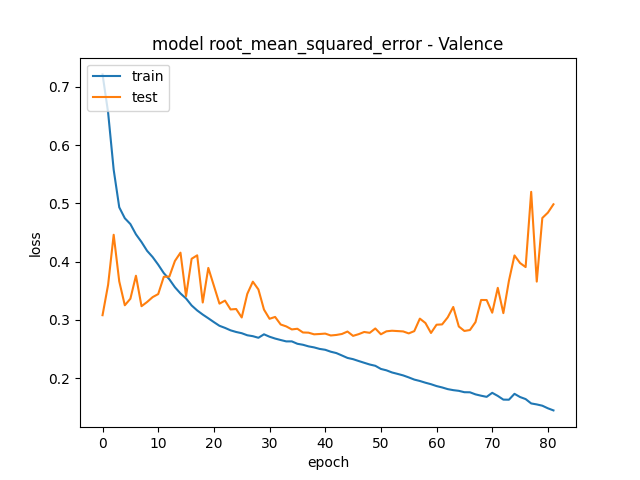
\includegraphics[angle=0, width=0.6\textwidth]{Figures/rmse_out1_L2Dense.png}
%   \caption{Applying L2 regularization to the classifier ends up in increasing the validation loss over time.}
%   \label{fig:AblationL2Dense}
%   \end{center}
% \end{figure}

% As it can be seen from the graph above, the application of L2 regularization to the Dense layer performed initially well on the validation/test data, like in the base model. However, toward later epochs, the validation/test loss started to increase which likely indicates overfitting of the model. The results for this approach can be summarized as follows:

% \begin{table}[H]
% \begin{center}
% \begin{tabular}{@{}lcccc@{}}
% \toprule
% \multicolumn{1}{c}{} & \begin{tabular}[c]{@{}c@{}}RMSE $\downarrow$\\ Valence\end{tabular} & \begin{tabular}[c]{@{}c@{}}RMSE $\downarrow$\\ Arousal\end{tabular} & \begin{tabular}[c]{@{}c@{}}CORR $\uparrow$\\ Valence\end{tabular} & \begin{tabular}[c]{@{}c@{}}CORR $\uparrow$\\ Arousal\end{tabular} \\ \midrule
% \begin{tabular}[c]{@{}l@{}}Multi-Phased FT\\ (no Data Aug.)\end{tabular} & 0.29 & 0.25 & -0.10 & 0.12 \\
% \begin{tabular}[c]{@{}l@{}}Multi-Phased FT\\ L2-Reg. Dense Layer\end{tabular} & \textbf{0.28} & 0.25 & -0.10 & \textbf{0.13} \\ \bottomrule
% \end{tabular}
% \caption{The slight performance gain through the application of L2 regularization to the classifier can be classified as negligible.}
% \label{tab:MPFTL2RegDense}
% \end{center}
% \end{table}

% Surprisingly, the model performed slightly better with L2 regularization in the classifier. However, due to the almost negligible improvement, it cannot be ascertained weather the improvement did occur just by chance.
% \newline\newline
% Another promising approach was the application of L2 regularization to all trainable (=unfrozen) layers from the pretrained VGGFace network, without applying it to the model's Dense layer. The results achieved for a 0.01 regularizer for the RMSE metric for 'Valence' look like this:

% \begin{figure}[H]
%   \begin{center}
%   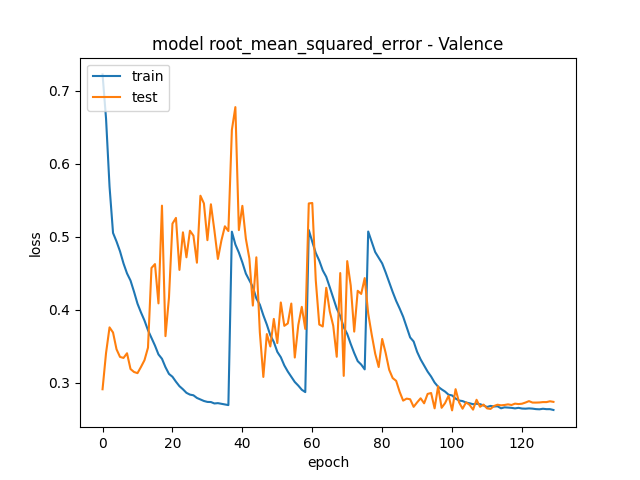
\includegraphics[angle=0, width=0.6\textwidth]{Figures/rmse_out1_L2VGGFace.png}
%   \caption{The application of L2 regularization to the pre-trained VGGFace model shows some promosing low test loss.}
%   \label{fig:AblationL2VGGFace}
%   \end{center}
% \end{figure}

% The curve, especially from the 90th epoch on, looks quite promising in terms of validation/test loss. However, the actual results obtained during the evaluation of the model on a separate test set showed substantially lower numbers for RMSE. The results are summarized and compared in the table below.

% \begin{table}[H]
% \begin{center}
% \begin{tabular}{@{}lcccc@{}}
% \toprule
% \multicolumn{1}{c}{} & \begin{tabular}[c]{@{}c@{}}RMSE $\downarrow$\\ Valence\end{tabular} & \begin{tabular}[c]{@{}c@{}}RMSE $\downarrow$\\ Arousal\end{tabular} & \begin{tabular}[c]{@{}c@{}}CORR $\uparrow$\\ Valence\end{tabular} & \begin{tabular}[c]{@{}c@{}}CORR $\uparrow$\\ Arousal\end{tabular} \\ \midrule
% \begin{tabular}[c]{@{}l@{}}Multi-Phased FT\\ (no Data Aug.)\end{tabular} & \textbf{0.29} & \textbf{0.25} & -0.10 & \textbf{0.12} \\
% \begin{tabular}[c]{@{}l@{}}Multi-Phased FT\\ L2-Reg. VGG Layer\end{tabular} & 0.40 & 0.28 & \textbf{-0.07} & 0.03 \\ \bottomrule
% \end{tabular}
% \caption{Evaluation results disprove the initial assumption that the performance might increase when applying L2 regularization to the pre-trained VGGFace network.}
% \label{tab:MPFTL2RegVGG}
% \end{center}
% \end{table}

% In summary, it could be proven that various regularization techniques, such as Dropout and Batch Normalization improved the proposed model's generalization capabilities. However, in the case of applying L2 weight regularization to either Dense or pre-trained Convolutional layers, was no substantial performance to be gained. On the contrary, it increased the validation, as well as the testing loss for both Valence and Arousal.

% %%%%%%%%%%%%%%%%%%%%%%%%%%%%%%%%%%%%%%%%%%%%%%%%%%%%%%%%%%%%%%%%
% \subsection{Recurrent Neural Network}
% % \textbf{- Can an LSTM capture the time-spatio changes between frames and thus enhance the performance of \gls{ER}}
% % Data needs to be non-shuffled in order to do that
% % -> Performance didn't increase

% The idea behind applying a Recurrent Neural Network (RNNs) is to capture the time-spatial changes in between frames with the goal of further enhancing the performance of emotion recognition. The specific type of RNN applied is callled LSTM. Additionally, the model's architecture needed to be changed in order to allow for an input of sequences with 5 frames each. These are fed into the model and processed simultaneously, going through the CNN, then the LSTM layer and finally the classifier. Moreover, frames inside the dataset mustn't be shuffled in order to be able to capture time-spatial changes.
% \newline\newline
% Results achieved in terms of RMSE metric of 'Valence' with an LSTM layer look like this:

% \begin{figure}[H]
%   \begin{center}
%   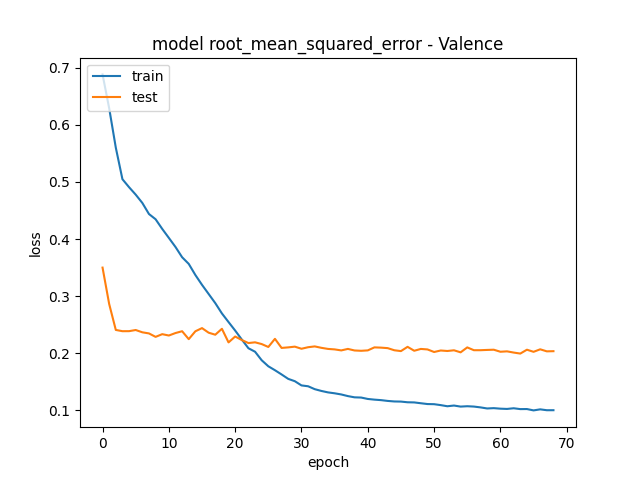
\includegraphics[angle=0, width=0.6\textwidth]{Figures/rmse_out_LSTM.png}
%   \caption{Using a LSTM layer shows a smooth curve, however, with a slow validation loss decrease.}
%   \label{fig:AblationLSTM}
%   \end{center}
% \end{figure}

% The following table compares the base model, with a CNN only architecture, to the proposed CNN + LSTM architecture. It shows that the LSTM performs better in terms of RMSE, but lacks in CORR, which makes it hard to judge whether it is really a better choice as CORR usually indicates the models' generalization ability. 

% \begin{table}[H]
% \begin{center}
% \begin{tabular}{lcc}
% \hline
% \multicolumn{1}{c}{Ablation study} & RMSE $\downarrow$ & CORR $\uparrow$ \\ \hline
% \begin{tabular}[c]{@{}l@{}}base model\\ (CNN only)\end{tabular} & 0.46 & \textbf{0.42} \\
% \begin{tabular}[c]{@{}l@{}}CNN + LSTM\\ (step size 3)\end{tabular} & \textbf{0.21} & 0.14 \\ \hline
% \end{tabular}
% \caption{Utilizing a LSTM layer in this experiment resulted in lower RMSE, but at the same time worse CORR.}
% \label{tab:LSTM}
% \end{center}
% \end{table}